% !TEX program = lualatex
\documentclass[paper=a4,fontsize=8pt,twocolumn]{jlreq}

\usepackage[top=11mm,bottom=12mm,left=12mm,right=12mm,columnsep=6mm]{geometry}
\usepackage{graphicx}
\usepackage{booktabs}
\usepackage{amsmath}
\usepackage{caption}
\usepackage{xcolor}
\usepackage{enumitem}
\usepackage{titlesec}

\captionsetup{font=footnotesize,labelfont=bf,skip=2pt}
\setlength{\parindent}{0.8em}
\setlength{\parskip}{0pt}
\setlength{\abovedisplayskip}{2pt}
\setlength{\belowdisplayskip}{2pt}
\setlength{\textfloatsep}{4pt}
\setlength{\floatsep}{4pt}
\setlength{\intextsep}{3pt}
\setlist[itemize]{leftmargin=1.1em,itemsep=0pt,topsep=1pt,parsep=0pt}
\titlespacing*{\section}{0pt}{0.45em}{0.25em}
\titlespacing*{\subsection}{0pt}{0.35em}{0.15em}
\titleformat{\section}{\bfseries\normalsize}{\thesection}{0.5em}{}
\titleformat{\subsection}{\bfseries\footnotesize}{\thesubsection}{0.4em}{}
\renewcommand{\arraystretch}{0.92}

\begin{document}

\twocolumn[
\begin{center}
{\Large\bfseries 低信頼エッジキャッシュ環境における近隣協調型フォールバック制御の初期検討}\\[-1mm]
{\small 進捗メモ（preliminary Monte Carlo simulation）\quad \today}
\vspace{1mm}

\begin{minipage}[t]{0.48\textwidth}
\centering
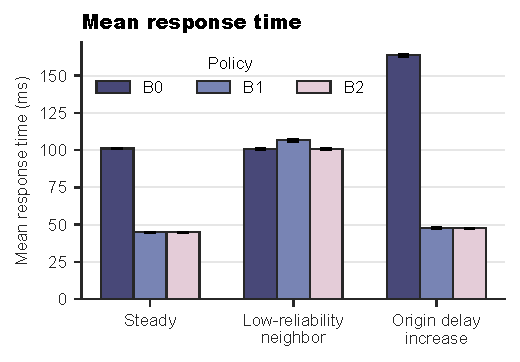
\includegraphics[width=\linewidth]{figures/fig_phase1_memo_scenario_mean_response_time.pdf}
\captionof{figure}{Mean response time. Error bars show 95\% confidence intervals.}
\end{minipage}
\hfill
\begin{minipage}[t]{0.48\textwidth}
\centering
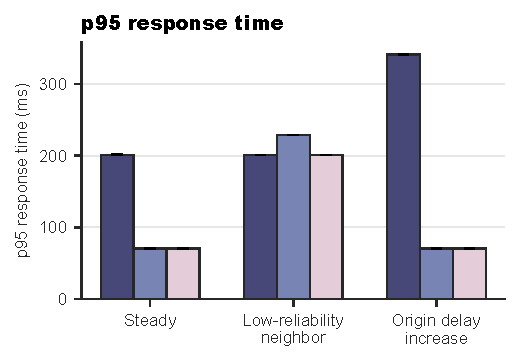
\includegraphics[width=\linewidth]{figures/fig_phase1_memo_scenario_p95_response_time.pdf}
\captionof{figure}{95th percentile response time.}
\end{minipage}
\end{center}
\vspace{-2mm}
]

\section{目的と方式}
本メモでは，ローカル ES 集合のみではファイル復元に必要なチャンク数を満たせない場合のフォールバック方式を比較した初期結果を報告する．現段階の評価は，正式な離散事象シミュレーションではなく，制御ロジックの傾向を確認する preliminary Monte Carlo simulation として位置づける．比較対象は以下の三方式である．

\begin{itemize}
  \item \textbf{B0}: ローカル復元失敗時，不足チャンクを直接オリジンから取得する．
  \item \textbf{B1}: ローカル復元失敗時，常に近隣 ES 協調グループを探索し，失敗時にオリジンへフォールバックする．
  \item \textbf{B2}: 期待遅延に基づく近隣探索判定方式であり，近隣探索が有利と推定される場合のみ近隣 ES を探索する．
\end{itemize}

B2 では，近隣復元成功確率を
$P_s=\Pr(X\ge K),\ X\sim\mathrm{Binomial}(N_{\mathrm{nbr}},p_{\mathrm{nbr}})$
と近似し，近隣探索の期待遅延を次式で判定する．
\[
E_{\mathrm{nbr}}
=P_sT_{\mathrm{nbr}}+(1-P_s)(T_{\mathrm{probe}}+T_{\mathrm{origin}})
\le T_{\mathrm{origin}} .
\]
条件を満たす場合は近隣探索を行い，満たさない場合は直接オリジン取得を選択する．

\section{実験設定}
要求は Zipf 分布（$\alpha=1.1$）に従うものとし，復元に必要なチャンク数は $K=3$，ローカル ES 数は 3，近隣 ES グループサイズは 5 とした．各条件で 10 trials，各 trial で 10,000 requests を用いた．評価指標は平均応答時間，95 パーセンタイル応答時間，オリジン非依存完了率，近隣探索失敗率である．

\begin{center}
\captionof{table}{代表シナリオの設定}
\footnotesize
\begin{tabular}{lccc}
\toprule
Scenario & Local & Neighbor & Origin delay \\
\midrule
定常 & 0.82 & 0.82 & 180 ms \\
低信頼近隣 ES & 0.82 & 0.25 & 180 ms \\
オリジン遅延増加 & 0.82 & 0.82 & 320 ms \\
\bottomrule
\end{tabular}
\end{center}
\vspace{-1mm}
低信頼近隣 ES シナリオの近隣 ES 可用率 0.25 は実測値ではなく，近隣探索が有効でない条件を観察するための stress setting である．また，ヒートマップでは，三つの代表シナリオで用いた近隣 ES 可用率およびオリジン遅延を含む範囲で感度分析を行った．

\section{初期結果}
定常シナリオでは，近隣 ES が十分利用可能であるため B1 と B2 はほぼ同等の性能を示した．これは，B2 の判定が多くの場合 B1 と同様に近隣探索を選択するためであり，baseline で B1/B2 の差が小さいことは自然な結果である．一方，低信頼近隣 ES シナリオでは，近隣復元成功確率が低く，近隣探索の期待遅延がオリジン取得遅延を上回るため，B2 は近隣探索を抑制する．そのため，B1 で生じる「近隣探索後に失敗し，その後オリジンへ戻る」二重の遅延負担を避ける傾向が見られた．オリジン遅延増加シナリオでは，近隣 ES が利用可能な条件では B1/B2 が B0 より低遅延となるが，B1 と B2 の差は小さい．

\begin{center}
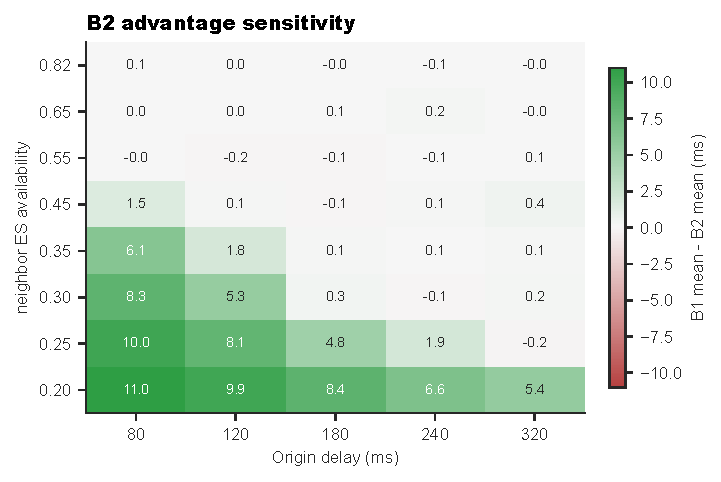
\includegraphics[width=0.88\columnwidth]{figures/fig_phase1_memo_b2_advantage_heatmap.pdf}
\captionof{figure}{補足的な感度分析として，近隣 ES 可用率とオリジン遅延を変化させた場合の B2 advantage を示す．B2 advantage = B1 mean response time $-$ B2 mean response time であり，正の値は B2 が B1 より低遅延であることを示す．}
\end{center}

\section{制限と次段階}
現在の B2 の $P_s$ は簡略化された確率モデルであり，request arrival，service capacity，queueing delay は含まない．したがって，オリジン遅延増加シナリオはオリジン取得遅延を増加させた stress setting であり，実際の server congestion を明示的にモデル化したものではない．また，content-level cache placement，cache capacity，cache replacement も未導入である．

次の段階では，コンテンツごとのキャッシュ配置やキャッシュ容量を導入する方向と，request arrival・service capacity・queueing delay を含む離散事象シミュレーションへ拡張する方向のどちらを優先すべきか，ご助言いただけますと幸いです．

\end{document}
